% Created 2018-06-21 Thu 12:30
\documentclass[8pt]{beamer}
\usepackage{pgfpages}

% ENABLE THIS FOR NOTES
%\setbeameroption{hide notes} % Only slides
%\setbeameroption{show only notes} % Only notes
\setbeameroption{show notes on second screen=right} % Both

\usepackage[sc,osf]{mathpazo}   % With old-style figures and real smallcaps.
\linespread{1.025}              % Palatino leads a little more leading
% Euler for math and numbers
\usepackage[euler-digits,small]{eulervm}
%\documentclass[10pt]{llncs}
%\usepackage{llncsdoc}
\usepackage{hyperref}
\usepackage{minted}
%\usemintedstyle{xcode}
\usepackage[utf8]{inputenc}
\usepackage[T1]{fontenc}
\usepackage{fixltx2e}
\usepackage{graphicx}
\usepackage{longtable}
\usepackage{float}
\usepackage{wrapfig}
\usepackage{rotating}
\usepackage[normalem]{ulem}
\usepackage{amsmath}
\usepackage{textcomp}
\usepackage{marvosym}
\usepackage{wasysym}
\usepackage{amssymb}
\usepackage{polynom}
\usepackage{changepage}
\usepackage{lipsum}


\hypersetup{colorlinks=true,
    linkcolor = blue,
    urlcolor  = blue,
    citecolor = blue,
    anchorcolor = blue
}
\renewcommand{\mod}[1]{\left( \texttt{mod}~#1 \right)}
\newcommand{\cpp}[1]{\mintinline{cpp}{#1}}
\newcommand{\py}[1]{\mintinline{py}{#1}}
\newcommand{\raw}[1]{\mintinline{text}{#1}}
\newcommand{\hs}[1]{\mintinline{hs}{#1}}
\newcommand{\smallpt}{\texttt{smallpt}}
\newcommand{\Ray}{\texttt{Ray}}
\newcommand{\Refl}{\texttt{Refl}}
\newcommand{\main}{\texttt{main}}
\newcommand{\intersect}{\texttt{intersect}}
\newcommand{\intersects}{\texttt{intersects}}
\tolerance=1000
% \usetheme{Antibes}
\author{Davean Scies, Siddharth Bhat}
\date{November 4th, 2020}
\institute{Haskell Exchange}
\title{Optimizing \smallpt}
\hypersetup{
  pdfkeywords={},
  pdfsubject={},
  pdfcreator={Emacs 24.5.1 (Org mode 8.2.10)}}

  \usepackage{xcolor}

\usepackage{listings}

\newcommand{\lstbg}[3][0pt]{{\fboxsep#1\colorbox{#2}{\strut #3}}}
\lstdefinelanguage{diff}{
  basicstyle=\ttfamily\small,
  morecomment=[f][\lstbg{red!20}]-,
  morecomment=[f][\lstbg{green!20}]+,
  morecomment=[f][\textit]{@@},
  %morecomment=[f][\textit]{---},
  %morecomment=[f][\textit]{+++},
}



\setbeamersize{text margin left=10pt,text margin right=5pt}


\begin{document}

\maketitle

\begin{frame}[fragile]{What is smallpt anyway?}
\pause
\begin{columns}
\begin{column}{0.48\textwidth}
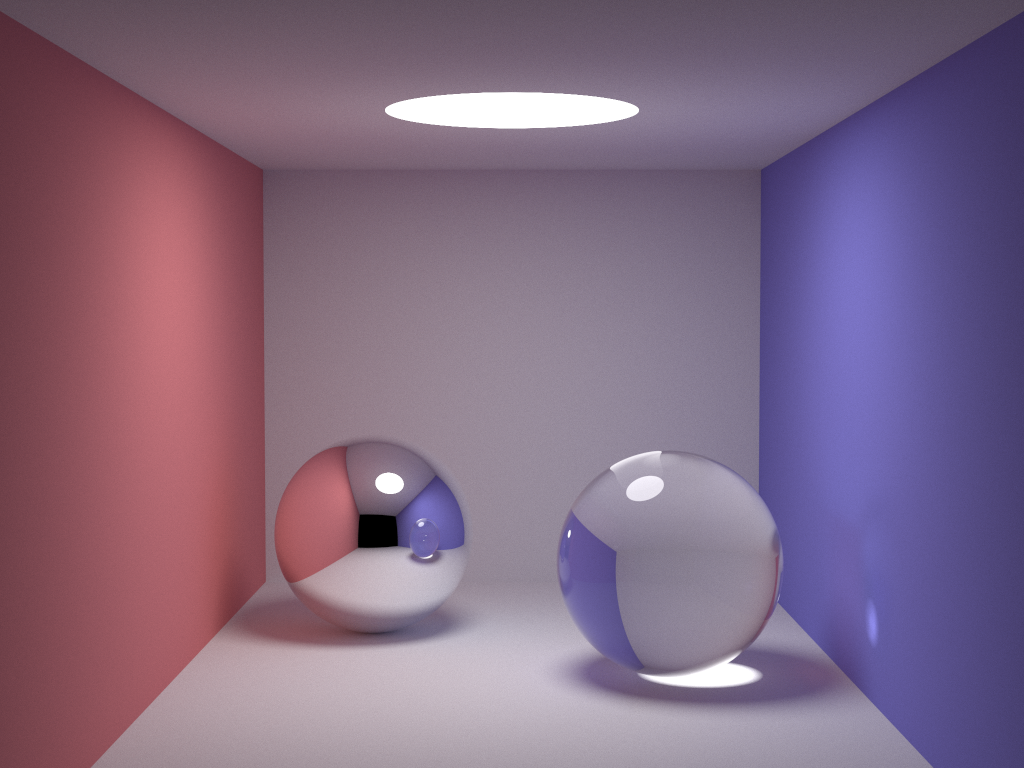
\includegraphics[height=0.8\textwidth]{./smallpt-render.png}
\end{column}
\begin{column}{0.48\textwidth}
\begin{itemize}
\item 99 LoC \texttt{C++}: \textbf{small}  \textbf{p}ath \textbf{t}racer.
\item Ported to many languages, including Haskell! (Thanks to Vo Minh Thu/\texttt{noteed}).
\item Start from \texttt{noteed}'s original source; SHA the output image from the Haskell source for baseline.
\end{itemize}
\end{column}
\end{columns}

\note[item]{\textbf{S}}
\note[item]{Perfect for an optimization case study.}
\note[item]{Plan: Quick walk through Haskell code, end up at \texttt{C++} (\texttt{clang++}) performance.}
\end{frame}

\begin{frame}[fragile]{What is smallpt anyway?}
% \begin{adjustwidth}{-5em}{-5em}
\begin{minted}{cpp}
struct Vec {      
  double x, y, z; // position, also color (r,g,b) 
  ... methods...
}; 
struct Ray { Vec o, d; Ray(Vec o_, Vec d_) : o(o_), d(d_) {} }; 
enum Refl_t { DIFF, SPEC, REFR };  // material types, used in radiance() 
struct Sphere { 
  double rad;   // radius 
  Vec p, e, c;  // position, emission, color 
  Refl_t refl;  // reflection type (DIFFuse, SPECular, REFRactive) 
  ... methods ...
  double intersect(const Ray &r) const // returns distance, 0 if nohit 
}; 
Sphere spheres[] = {//Scene: radius, position, emission, color, material 
  Sphere(1e5, Vec( 1e5+1,40.8,81.6), Vec(),Vec(.75,.25,.25),DIFF),//Left 
  ... initialization ...
}; 
\end{minted}
% \end{adjustwidth}
\note[item]{\textbf{S}}
\note[item]{Has geometric primitives: vectors, spheres, materials}
\note[item]{Entirely number-based, no real data structure}
\end{frame}


\begin{frame}[fragile]{What is smallpt anyway?}
\footnotesize
\begin{minted}{cpp}
Vec radiance(const Ray &r, int depth, unsigned short *Xi){ 
                                                                         
                                                                         
                                                                      
                                                               
                                                                           
                                                                            
                                                                            
                                                                         
                                                                   
                                                                     
                                                                      
                                                           
                                                                          
                                                                            
                                                                            
                                                                           
                                                                        
                                                                          
                                                          
                                                                          
                                                                           
                                                                            
                                                                            
                                                                          
                                                                         
} 
\end{minted}

\note[item]{\textbf{S}}
\note[item]{Most of the compute cost is spent in the function that traces rays.}
\note[item]{is called radiance}
\end{frame}


\begin{frame}[fragile]{What is smallpt anyway?}
\footnotesize
\begin{minted}{cpp}
Vec radiance(const Ray &r, int depth, unsigned short *Xi){ 
                                                                      
                                                                      
                                                                   
                                                            
                                                                        
                                                                         
                                       
                                          
                                                                
                                                                  
                                                                   
                          radiance
                                          
                          radiance
                                                                         
                                                                        
                                                                     
                                         
                          radiance
                                                                       
                                                                        
                                                                         
                                                                         
    radiance                      radiance
    radiance                      radiance
} 
\end{minted}
\note[item]{\textbf{S}}
\note[item]{Recursively calls itself a bunch of times}
\end{frame}

\begin{frame}[fragile]{What is smallpt anyway?}
\footnotesize
\begin{minted}{cpp}
Vec radiance(const Ray &r, int depth, unsigned short *Xi){ 
                                                                      
                                                                      
                                                                   
                                                            
                                                                        
                                                                         
  if (         ) if (             )            else 
  if (                ){                  
                                                                
                                                                  
                                                                   
                          radiance
  } else if (                )            
                          radiance
                                                                         
                                                                        
                                                                     
  if (                               )   
                          radiance
                                                                       
                                                                        
                                                                         
                                                                         
    radiance                      radiance
    radiance                      radiance
} 
\end{minted}
\note[item]{\textbf{S}}
\note[item]{Recursion is guarded by a lot of control flow}
\end{frame}


\begin{frame}[fragile]{What is smallpt anyway?}
\footnotesize
\begin{minted}{cpp}
Vec radiance(const Ray &r, int depth, unsigned short *Xi){ 
                                                                      
                                                                      
                                                                   
                                                            
  Vec x=r.o+r.d*t, n=(x-obj.p).norm(), nl=n.dot(r.d)<0?n:n*-1, f=obj.c; 
                                                                         
  if (         ) if (             )            else 
  if (                ){                  
                                                                
                                                                  
                                                                   
                          radiance
  } else if (                )            
                          radiance
                                                                         
                                                                        
                                                                     
  if ((cos2t=1-nnt*nnt*(1-ddn*ddn))<0)
                          radiance
                                                                       
                                                                        
                                                                         
                                                                         
    radiance                      radiance
    radiance                      radiance
} 
\end{minted}
\note[item]{\textbf{S}}
\note[item]{The control flow and computation is very numeric in nature}
\end{frame}

\begin{frame}[fragile]{What is smallpt anyway?}
\footnotesize
\begin{minted}{cpp}
Vec radiance(const Ray &r, int depth, unsigned short *Xi){ 
                                                                      
                                                                      
                                                                   
                                                            
  Vec x=r.o+r.d*t, n=(x-obj.p).norm(), nl=n.dot(r.d)<0?n:n*-1, f=obj.c; 
                                                                         
  if (         ) if (erand48(Xi)  )            else 
  if (                ){                  
                     erand48(Xi)     erand48(Xi)
                                                                  
                                                                   
                          radiance
  } else if (                )            
                          radiance
                                                                         
                                                                        
                                                                     
  if ((cos2t=1-nnt*nnt*(1-ddn*ddn))<0)
                          radiance
                                                                       
                                                                        
                                                                         
                                   erand48(Xi)
    radiance                      radiance
    radiance                      radiance
} 
\end{minted}
\note[item]{\textbf{S}}
\note[item]{We use erand48 for randomness}
\end{frame}


\begin{frame}[fragile]{What is smallpt anyway?}
\footnotesize
\begin{minted}{cpp}
Vec radiance(const Ray &r, int depth, unsigned short *Xi){ 
  double t;                               // distance to intersection 
  int id=0;                               // id of intersected object 
  if (!intersect(r, t, id)) return Vec(); // if miss, return black 
  const Sphere &obj = spheres[id];        // the hit object 
  Vec x=r.o+r.d*t, n=(x-obj.p).norm(), nl=n.dot(r.d)<0?n:n*-1, f=obj.c; 
  double p = f.x>f.y && f.x>f.z ? f.x : f.y>f.z ? f.y : f.z; // max refl 
  if (++depth>5) if (erand48(Xi)<p) f=f*(1/p); else return obj.e; //R.R. 
  if (obj.refl == DIFF){                  // Ideal DIFFUSE reflection 
    double r1=2*M_PI*erand48(Xi), r2=erand48(Xi), r2s=sqrt(r2); 
    Vec w=nl, u=((fabs(w.x)>.1?Vec(0,1):Vec(1))%w).norm(), v=w%u; 
    Vec d = (u*cos(r1)*r2s + v*sin(r1)*r2s + w*sqrt(1-r2)).norm(); 
    return obj.e + f.mult(radiance(Ray(x,d),depth,Xi)); 
  } else if (obj.refl == SPEC)            // Ideal SPECULAR reflection 
    return obj.e + f.mult(radiance(Ray(x,r.d-n*2*n.dot(r.d)),depth,Xi)); 
  Ray reflRay(x, r.d-n*2*n.dot(r.d));     // Ideal dielectric REFRACTION 
  bool into = n.dot(nl)>0;                // Ray from outside going in? 
  double nc=1, nt=1.5, nnt=into?nc/nt:nt/nc, ddn=r.d.dot(nl), cos2t; 
  if ((cos2t=1-nnt*nnt*(1-ddn*ddn))<0)    // Total internal reflection 
    return obj.e + f.mult(radiance(reflRay,depth,Xi)); 
  Vec tdir = (r.d*nnt - n*((into?1:-1)*(ddn*nnt+sqrt(cos2t)))).norm(); 
  double a=nt-nc, b=nt+nc, R0=a*a/(b*b), c = 1-(into?-ddn:tdir.dot(n)); 
  double Re=R0+(1-R0)*c*c*c*c*c,Tr=1-Re,P=.25+.5*Re,RP=Re/P,TP=Tr/(1-P); 
  return obj.e + f.mult(depth>2 ? (erand48(Xi)<P ?   // Russian roulette 
    radiance(reflRay,depth,Xi)*RP:radiance(Ray(x,tdir),depth,Xi)*TP) : 
    radiance(reflRay,depth,Xi)*Re+radiance(Ray(x,tdir),depth,Xi)*Tr); 
} 
\end{minted}
\note[item]{\textbf{S}}
\note[item]{The full code continues to be more of the same}
\end{frame}


\begin{frame}[fragile]{Initial Haskell Code: \texttt{radiance} ($1\times$)}
% 620027b45e40e5a4b18f36cabc70efe803f41a61
\begin{minted}[fontsize=\tiny]{hs}
radiance :: Ray -> CInt -> Ptr CUShort -> IO Vec
radiance ray@(Ray o d) depth xi = case intersects ray of
  (Nothing,_) -> return zerov
  (Just t,Sphere _r p e c refl) -> do
                                        
                                   
                                                              
                         
                                
        continue f = case refl of - BRANCHING
          DIFF -> do
            r1 <- ((2*pi)*) `fmap` erand48 xi -- RNG
                                                
                               
                                
                                      
                                                                                           
                                  
                                                                                                                
                   radiance 
                                            
          SPEC -> do
                                                         
            rad <- radiance  -- RECURSION
                                            
          REFR -> do
                                                                                                     
                                                                                   
                         
                           
                                                      
                                
                                                
            if 
              then do
                rad <- radiance
            ...
\end{minted}

\note[item]{\textbf{S}}
\note[item]{the original source has the same computation in haskell}
% \raw{Sha256} hash of the output image --- \raw{4dac691082bb}
\end{frame}


\begin{frame}[fragile]{Initial Haskell Code: Data structures}
\begin{minted}[fontsize=\small]{hs}
data Vec = Vec {-# UNPACK #-} !Double {-# UNPACK #-} !Double {-# UNPACK #-} !Double

cross :: Vec -> Vec -> Vec
(.*) :: Vec -> Double -> Vec
infixl 7 .*
len :: Vec -> Double
norm :: Vec -> Vec
norm v = v .* recip (len v)
dot :: Vec -> Vec -> Double
maxv :: Vec -> Double

data Ray = Ray Vec Vec -- origin, direction
data Refl = DIFF | SPEC | REFR -- material types, used in radiance
-- | radius, position, emission, color, reflection
data Sphere = Sphere Double Vec Vec Vec Refl
\end{minted}

\note[item]{\textbf{S}}
\note[item]{We implement the same data structures in Haskell}
\note[item]{Note that \texttt{Ray, Sphere} not having unpack}
\end{frame}

\begin{frame}[fragile]{Initial Haskell Code: scene data}
\begin{minted}[fontsize=\small]{hs}
spheres :: [Sphere]
spheres =
  [ Sphere 1e5  (Vec (1e5+1) 40.8 81.6)  0 (Vec 0.75 0.25 0.25) DIFF --Left
  , Sphere 1e5  (Vec (99-1e5) 40.8 81.6) 0 (Vec 0.25 0.25 0.75) DIFF --Rght
  , Sphere 1e5  (Vec 50 40.8 1e5)        0 0.75  DIFF --Back
  , Sphere 1e5  (Vec 50 40.8 (170-1e5))  0 0     DIFF --Frnt
  , Sphere 1e5  (Vec 50 1e5 81.6)        0 0.75  DIFF --Botm
  , Sphere 1e5  (Vec 50 (81.6-1e5) 81.6) 0 0.75  DIFF --Top
  , Sphere 16.5 (Vec 27 16.5 47)         0 0.999 SPEC --Mirr
  , Sphere 16.5 (Vec 73 16.5 78)         0 0.999 REFR --Glas
  , Sphere 600  (Vec 50 681.33 81.6)    12 0     DIFF]--Lite
\end{minted}

\note[item]{\textbf{S}}
\note[item]{this list will be walked many times, as it contains our scene information.}
\end{frame}

\begin{frame}[fragile]{Initial Haskell code: Sphere intersection}
\begin{minted}{hs}
intersect :: Ray -> Sphere -> Maybe Double
intersect (Ray o d) (Sphere r p _e _c _refl) =
  if det<0 then Nothing else f (b-sdet) (b+sdet)
  where op = p - o -- Numeric
        eps = 1e-4
        b = dot op d
        det = b*b - dot op op + r*r -- Numeric
        sdet = sqrt det
        f a s = if a>eps then Just a else if s>eps then Just s else Nothing
intersects :: Ray -> (Maybe Double, Sphere)
intersects ray = (k, s)
  where (k,s) = foldl' f (Nothing,undefined) spheres -- Spheres iterated over
        f (k',sp) s' = case (k',intersect ray s') of
                  (Nothing,Just x) -> (Just x,s')
                  (Just y,Just x) | x < y -> (Just x,s')
                  _ -> (k',sp)
\end{minted}
\note[item]{\textbf{S}}
\note[item]{Responsible for figuring out what the ray hits.}
\note[item]{We iterate over the list of spheres.}
\note[item]{Once again, numeric heavy.}
\note[item]{Use a Maybe to indicate whether we've found an answer or not.}
\end{frame}

\begin{frame}[fragile]{Initial Haskell Code: \texttt{radiance} ($1\times$) }
% 620027b45e40e5a4b18f36cabc70efe803f41a61
\begin{minted}[fontsize=\tiny]{hs}
radiance :: Ray -> CInt -> Ptr CUShort -> IO Vec
radiance ray@(Ray o d) depth xi = case intersects ray of
  (Nothing,_) -> return zerov
  (Just t,Sphere _r p e c refl) -> do
    let x = o `addv` (d `mulvs` t)
        n = norm $ x `subv` p
        nl = if n `dot` d < 0 then n else n `mulvs` (-1)
        pr = maxv c
        depth' = depth + 1
        continue f = case refl of
          DIFF -> do
            r1 <- ((2*pi)*) `fmap` erand48 xi
            r2 <- erand48 xi
            let r2s = sqrt r2
                w@(Vec wx _ _) = nl
                u = norm $ (if abs wx > 0.1 then (Vec 0 1 0) else (Vec 1 0 0)) `cross` w
                v = w `cross` u
                d' = norm $ (u`mulvs`(cos r1*r2s)) `addv` (v`mulvs`(sin r1*r2s)) `addv` (w`mulvs`sqrt (1-r2))
            rad <- radiance (Ray x d') depth' xi
            return $ e `addv` (f `mulv` rad)
          SPEC -> do
            let d' = d `subv` (n `mulvs` (2 * (n`dot`d)))
            rad <- radiance (Ray x d') depth' xi
            return $ e `addv` (f `mulv` rad)
          REFR -> do
            let reflRay = Ray x (d `subv` (n `mulvs` (2* n`dot`d)))
                into = n`dot`nl > 0                
                nc = 1
                nt = 1.5
                nnt = if into then nc/nt else nt/nc
                ddn= d`dot`nl
                cos2t = 1-nnt*nnt*(1-ddn*ddn)
            if cos2t<0
              then do
                rad <- radiance reflRay depth' xi
            ...
\end{minted}
% \raw{Sha256} hash of the output image --- \raw{4dac691082bb}

\note[item]{\textbf{S}}
\note[item]{Branch heavy}
\note[item]{Recursive}
\note[item]{Uses an RNG}
\end{frame}



\begin{frame}[fragile]{Initial Haskell Code: Entry point  ($1\times$)}
\begin{minted}{hs}
smallpt :: Int -> Int -> Int -> IO ()
smallpt w h nsamps = do
  ...
  c <- VM.replicate (w * h) 0
  allocaArray 3 \xi -> -- Create mutable memory
    flip mapM_ [0..h-1] $ \y -> do -- Loop
      writeXi xi y
      for_ [0..w-1] \x -> do -- Loop
        let i = (h-y-1) * w + x
        for_ [0..1] \sy -> do -- Loop
          for_ [0..1] \sx -> do -- Loop
            r <- newIORef 0 -- Create mutable memory
            for_ [0..samps-1] \_s -> do -- Loops, Loops
              r1 <- (2*) <$> erand48 xi
              ...
              rad <- radiance (Ray (org+d.*140) (norm d)) 0 xi  -- Crunch
              ...
              modifyIORef r (+ rad .* recip (fromIntegral samps)) -- Write
            ci <- VM.unsafeRead c i
            Vec rr rg rb <- readIORef r
            VM.unsafeWrite c i $ 
                ci + Vec (clamp rr) (clamp rg) (clamp rb) .* 0.25 -- Write
            ...
\end{minted}

\note[item]{\textbf{S}}
\note[item]{Uses mutability}
\note[item]{Performs number crunchy loops}
\note[item]{Finally, writes results out}
\end{frame}

\begin{frame}[fragile]{Initial Haskell Code: File I/O  ($1\times$)}
\begin{minted}{hs}
  withFile "image.ppm" WriteMode $ \hdl -> do
        hPrintf hdl "P3\n%d %d\n%d\n" w h (255::Int)
        flip mapM_ [0..w*h-1] \i -> do
          Vec r g b <- VM.unsafeRead c i
          hPrintf hdl "%d %d %d " (toInt r) (toInt g) (toInt b)
\end{minted}
% \note[item]{Point out the use of printf}
\end{frame}

\begin{frame}[fragile]{Initial Haskell Code: RNG ($1\times$)}
\begin{minted}{hs}
foreign import ccall unsafe "erand48"
  erand48 :: Ptr CUShort -> IO Double
\end{minted}
\note[item]{\textbf{S}}
\note[item]{We use the RNG to decide randomly in which direction to send rays}
\note[item]{Point out the use of foreign CCall.}
\end{frame}


\begin{frame}[fragile]{Restrict export list to `main` ($1.13\times$)}
% 4678326cbb78368977f901ed32e0bdb55b8be6c7
\begin{minted}{diff}
-module Main where
+module Main (main) where
\end{minted}

\pause
\begin{itemize}
\item Exported functions could be used by something unknown.
\item Original versions must be available.
\end{itemize}
\note[item]{\textbf{S}}
\note[item]{The very first thing to do is to let the compiler actually optimize.}
\note[item]{Compiler can't know how exported functions are used.}
\note[item]{Export lists not just about encapsulation.}
\end{frame}


\begin{frame}[fragile]{Mark entries of Ray and Sphere as UNPACK and Strict ($1.07\times$)}
% 1ad231a927f1a0582aee3f161e91372f7124d0c7

\begin{minted}[fontsize=\small]{diff}
data Vec = Vec {-# UNPACK #-} !Double 
               {-# UNPACK #-} !Double 
               {-# UNPACK #-} !Double

-data Ray = Ray Vec Vec -- origin, direction
+data Ray = Ray {-# UNPACK #-} !Vec {-# UNPACK #-} !Vec -- origin, direction

 data Refl = DIFF | SPEC | REFR -- material types, used in radiance

 -- radius, position, emission, color, reflection
-data Sphere = Sphere Double Vec Vec Vec !Refl
+data Sphere = Sphere {-# UNPACK #-} !Double 
+                     {-# UNPACK #-} !Vec 
+                     {-# UNPACK #-} !Vec 
+                     {-# UNPACK #-} !Vec !Refl
\end{minted}

\begin{minted}[fontsize=\small]{cpp}
struct Vec { double x, y, z; }
struct Ray { std::function<Vec()> v; std::function<Vec()> w; };
struct RayUnpack { double xv, yv, int zv;
                   double xw, yw, zw; };
\end{minted}

\note[item]{\textbf{D}}
\note[item]{Strictness in the arguments means that they're evaluated when instantiated, not when demanded. }
\note[item]{Where as Unpacking removes indirection from doing a memory lookup for components.}
\note[item]{Means we have to copy everything into the data structure that it is unpacked into.}
\note[item]{We don't unpack ray (Lots of calculations on its components, want those to fuse)}
\note[item]{Unpack Sphere - its static from compile time}
\note[item]{Don't unpack Ray, because each Vec undergoes a lot of computation.}
\end{frame}

\begin{frame}[fragile]{Use a pattern synonym to unpack Refl in Sphere ($1.07\times$)}
% e1819a6

\begin{minted}[fontsize=\small]{diff}
+{-# LANGUAGE PatternSynonyms #-}
\end{minted}


\begin{minted}[fontsize=\small]{diff}
-data Refl = DIFF | SPEC | REFR -- material types, used in radiance
+newtype Refl = Refl Int  -- material types, used in radiance
+pattern DIFF,SPEC,REFR :: Refl
+pattern DIFF = Refl 0
+pattern SPEC = Refl 1
+pattern REFR = Refl 2
+{-# COMPLETE DIFF, SPEC, REFR #-}

 -- radius, position, emission, color, reflection
 data Sphere = Sphere {-# UNPACK #-} !Double 
                      {-# UNPACK #-} !Vec
                      {-# UNPACK #-} !Vec 
-                     {-# UNPACK #-} !Vec !Refl
+                     {-# UNPACK #-} !Vec {-# UNPACK #-} !Refl

 \end{minted}


\note[item]{\textbf{D}}
\note[item]{Was unable to unpack Refl}
\note[item]{UnboxedSums are recent}
\note[item]{UnboxedSums are very unpleasant}
\note[item]{We're using an older trick to fake the unboxing here instead.}
\note[item]{In this case it isn't much of a win, but it illustrates the technique.}

\end{frame}

\begin{frame}[fragile]{Change from \texttt{maximum} on a list to \texttt{max} ($1.08\times$)}
% e77b26f
\begin{minted}{diff}
-maxv (Vec a b c) = maximum [a,b,c]
+maxv (Vec a b c) = max a (max b c)
\end{minted}

\begin{minted}{diff}
     let x = o `addv` (d `mulvs` t)
         n = norm $ x `subv` p
         nl = if n `dot` d < 0 then n else n `mulvs` (-1)
-        pr = maxv c
         depth' = depth + 1
         continue f = case refl of
           DIFF -> do
...
     if depth'>5
       then do
         er <- erand48 xi
+        let !pr = maxv c
\end{minted}

\note[item]{\textbf{D}}
\note[item]{Prebuild comparison}
\note[item]{Don't go via list}
\note[item]{GHC does not evaluate at compile time, only has RULES}
\note[item]{Doesn't really help much in this case}
\end{frame}

\begin{frame}[fragile]{Convert \texttt{erand48} to pure Haskell ($1.09\times$)}
% 48aeb46
\begin{minted}[fontsize=\small]{diff}
-foreign import ccall unsafe "erand48"
-  erand48 :: Ptr CUShort -> IO Double

+erand48 :: IORef Word64 -> IO Double
+erand48 !t =  do -- | Some number crunchy thing.
+  r <- readIORef t
+  let x' = 0x5deece66d * r + 0xb
+      d_word = 0x3ff0000000000000 .|. ((x' .&. 0xffffffffffff) `unsafeShiftL` 4)
+      d = castWord64ToDouble d_word - 1.0
+  writeIORef t x'
+  pure d
...
-radiance :: Ray -> CInt -> Ptr CUShort -> IO Vec
+radiance :: Ray -> Int -> IORef Word64 -> IO Vec -- IORef with state
 radiance ray@(Ray o d) depth xi = case intersects ray of
   ...
   c <- VM.replicate (w * h) zerov
-  allocaArray 3 $ \xi -> -- Old RNG state
-      flip mapM_ [0..h-1] $ \y -> do
+  xi <- newIORef 0 -- New RNG state
+  flip mapM_ [0..h-1] $ \y -> do
       writeXi xi y
\end{minted}

\note[item]{\textbf{S}}
\note[item]{The entire premise of this talk is that Haskell can be as fast as C.}
\note[item]{We're opening the black box of what erand48 does to GHC}
\note[item]{Further any impedance mismatch, such as FFI almost universally has to have, carries some bookkeeping overhead. }
\note[item]{If our Haskell code was as fast as the C code moving the code into Haskell would be a win, if it was slightly slower it could still be a win.}
\note[item]{Often considering your Haskell code's performance is a better option and easier than reimplementing something in C.}
\note[item]{As is the way with optimizations, this is not universally true.}
\end{frame}

\begin{frame}[fragile]{Remove mutability: \texttt{Erand48} Monad}


\begin{minted}[fontsize=\small]{diff}
-erand48 :: IORef Word64 -> IO Double
-erand48 !t =  do
-  r <- readIORef t
+data ET a = ET !Word64 !a deriving Functor
+newtype Erand48 a = Erand48 { runErand48' :: Word64 -> ET a } deriving Functor
+instance Applicative Erand48 where
+instance Monad Erand48 where
+runWithErand48 :: Int -> Erand48 a -> a                                                                                                
+erand48 :: Erand48 Double
...
-radiance :: Ray -> Int -> IORef Word64 -> IO Vec
-radiance ray@(Ray o d) depth xi = case intersects ray of
+radiance :: Ray -> Int -> Erand48 Vec
+radiance ray@(Ray o d) depth = case intersects ray of
...
-            r1 <- (2*pi*) <$> erand48 xi
-            r2 <- erand48 xi
+            r1 <- (2*pi*) <$> erand48
+            r2 <- erand48
...
-                              then (.* rp) <$> radiance reflRay depth' xi
-                              else (.* tp) <$> radiance (Ray x tdir) depth' xi
+                              then (.* rp) <$> radiance reflRay depth'
+                              else (.* tp) <$> radiance (Ray x tdir) depth'
\end{minted}

\note[item]{\textbf{D}}
\note[item]{All these mutability locations throw in extra RTS code, extra sequencing that blocks the compiler's optimization, and dependency chains.}
\note[item]{Sometimes we need mutability for performance.}
\note[item]{SSA is normal to compilers though.}
\note[item]{We almost start at SSA as a functional language.}
\note[item]{don't break it when you don't have a good reason.}

\end{frame}

\begin{frame}[fragile]{Removing mutation: eliminate \texttt{IORef} and \texttt{Data.Vector.Mutable}}
\begin{minted}[fontsize=\small]{diff}
-  c <- VM.replicate (w * h) 0
-  xi <- newIORef 0
-  flip mapM_ [0..h-1] $ \y -> do
-      writeXi xi y
-      for_ [0..w-1] \x -> do
-        let i = (h-y-1) * w + x
-        for_ [0..1] \sy -> do
-          for_ [0..1] \sx -> do
-            r <- newIORef 0
-            for_ [0..samps-1] \_s -> do
-              r1 <- (2*) <$> erand48 xi
+      img = (`concatMap` [(h-1),(h-2)..0]) $ \y -> runWithErand48 y do
+        for [0..w-1] \x -> do
+          (\pf -> foldlM pf 0 [(sy, sx) | sy <- [0,1], sx <- [0,1]]) \ci (sy, sx) -> do
+            Vec rr rg rb <- (\f -> foldlM f 0 [0..samps-1]) \ !r _s -> do
+              r1 <- (2*) <$> erand48
...
-              modifyIORef r (+ rad .* recip (fromIntegral samps))
-            ci <- VM.unsafeRead c i
-            Vec rr rg rb <- readIORef r
-            VM.unsafeWrite c i $ ci + Vec (clamp rr) (clamp rg) (clamp rb) .* 0.25
+              pure (r + rad .* recip (fromIntegral samps))
+            pure (ci + Vec (clamp rr) (clamp rg) (clamp rb) .* 0.25)
...
\end{minted}


\note[item]{\textbf{D}}

\end{frame}


\begin{frame}[fragile]{Set \textbf{everything} in \texttt{smallpt} to be strict ($1.17\times$)}
% e62177b
\begin{minted}[fontsize=\small]{diff}
smallpt :: Int -> Int -> Int -> IO ()
smallpt w h nsamps = do
-  let samps = nsamps `div` 4
-      org = Vec 50 52 295.6
-      dir = norm $ Vec 0 (-0.042612) (-1)
-      cx = Vec (fromIntegral w * 0.5135 / fromIntegral h) 0 0
-      cy = norm (cx `cross` dir) `mulvs` 0.5135
+  let !samps = nsamps `div` 4
+      !org = Vec 50 52 295.6
+      !dir = norm $ Vec 0 (-0.042612) (-1)
+      !cx = Vec (fromIntegral w * 0.5135 / fromIntegral h) 0 0
+      !cy = norm (cx `cross` dir) `mulvs` 0.5135
...
-  r1 <- (2*) `fmap` erand48 xi
-  let dx = if r1<1 then sqrt r1-1 else 1-sqrt(2-r1)
-  r2 <- (2*) `fmap` erand48 xi
-  let dy = if r2<1 then sqrt r2-1 else 1-sqrt(2-r2)
-      d = ...
-  rad <- radiance (Ray (org`addv`(d`mulvs`140)) (norm d)) 0 xi
+  !r1 <- (2*) `fmap` erand48 xi
+  let !dx = if r1<1 then sqrt r1-1 else 1-sqrt(2-r1)
+  !r2 <- (2*) `fmap` erand48 xi
+  let !dy = if r2<1 then sqrt r2-1 else 1-sqrt(2-r2)
+      !d = ...
...
+              pure $! r + rad .* recip (fromIntegral samps)
+            pure $! ci + Vec (clamp rr) (clamp rg) (clamp rb) .* 0.25
\end{minted}

\note[item]{\textbf{D}}
\note[item]{This is not a recommendation, this is a warning.}
\note[item]{We get a speedup here but it can also regress performance. Some of these bangs are regressions that are hidden.}
\note[iem]{Don't senselessly bang everything in sight. }

\end{frame}

\begin{frame}[fragile]{Why strictness may be bad}
\begin{minted}[fontsize=\small]{hs}
let foo = let x = error "ERR" in \y -> y
let foo' = let !x = error "ERR" in \y -> y
\end{minted}
\pause
\begin{minted}[fontsize=\small]{hs}
let fooOpt = \y -> y
let foo'Opt = \y -> y  -- ERROR! forcing foo' should give "ERR"
\end{minted}
% \pause
% \begin{minted}[fontsize=\small]{hs}
% let tuple = (42, error "urk")
% let bar = let (x, y) = tuple in \z -> x + z
% \end{minted}
% \pause
% \begin{minted}[fontsize=\small]{hs}
% let barOpt = \z -> 42 + z
% \end{minted}
% \pause
% \begin{minted}[fontsize=\small]{hs}
% let bar' = let (x, !y) = tuple in \z -> x + z
% \end{minted}
% \pause
% \begin{minted}[fontsize=\small]{hs}
% let bar'Opt =  \z -> 42 + z  --  ERROR: forcing bar' should give "urk"
% \end{minted}
\note[item]{\textbf{S}}
\note[item]{bangs remove freedom from the compiler}
\note[item]{bangs force large objects to be evaluated}
\note[item]{Haskell is awesome because equational reasoning.}
\note[item]{Bangs are not great with equational reasoning.}
\note[item]{judiciously use bangs. Too many remove choice from the compiler.}
\end{frame}


\begin{frame}[fragile]{Reduce to only useful strictnesses in \texttt{smallpt}($1.17\times$)}
\begin{minted}{diff}
-  let !samps = nsamps `div` 4
-      !org = Vec 50 52 295.6
-      !dir = norm $ Vec 0 (-0.042612) (-1)
-      !cx = Vec (fromIntegral w * 0.5135 / fromIntegral h) 0 0
-      !cy = norm (cx `cross` dir) .* 0.5135
+  let samps = nsamps `div` 4
+      org = Vec 50 52 295.6
+      dir = norm $ Vec 0 (-0.042612) (-1)
+      cx = Vec (fromIntegral w * 0.5135 / fromIntegral h) 0 0
+      cy = norm (cx `cross` dir) .* 0.5135
...
-              !r1 <- (2*) <$> erand48
+              r1 <- (2*) <$> erand48
...
-              !r2 <- (2*) <$> erand48
+              r2 <- (2*) <$> erand48
...
-              !rad <- radiance (Ray (org+d.*140) (norm d)) 0
+              rad <- radiance (Ray (org+d.*140) (norm d)) 0
...
-              pure $! r + rad .* recip (fromIntegral samps)
-            pure $! ci + Vec (clamp rr) (clamp rg) (clamp rb) .* 0.25
+              pure (r + rad .* recip (fromIntegral samps))
+            pure (ci + Vec (clamp rr) (clamp rg) (clamp rb) .* 0.25)
\end{minted}

\note[item]{\textbf{D}}
\note[item]{Thus the compiler can no longer move the computation around or simplify it.}
\note[item]{Force useless work.}
\note[item]{A little thinking about how the variables are used or looking at core allows us to select which ones we bang selectively.}
\end{frame}

\begin{frame}[fragile]{Use strictness strategically in entire project}
\begin{minted}[fontsize=\small]{diff}
...
-  if det<0 then Nothing else f (b-sdet) (b+sdet)
-  where op = p - o
-        eps = 1e-4
-        b = dot op d
-        det = b*b - dot op op + r*r
-        sdet = sqrt det
-        f a s = if a>eps then Just a else if s>eps then Just s else Nothing
+  if det<0
+  then Nothing
+  else
+    let !eps = 1e-4
+        !sdet = sqrt det
+        !a = b-sdet
+        !s = b+sdet
+    in if a>eps then Just a else if s>eps then Just s else Nothing
...
\end{minted}

\note[item]{\textbf{D}}
\note[item]{Sometimes (point out 'intersect') we have to rearrange the code though when we use bangs.}
\note[item]{Bangs tell the compiler to make more efficient code, but take away the compiler's options in how to do so.}
\note[item]{Only take away the compiler's liberties when it's using them poorly.}
\note[item]{Becomes intuitive.}

\end{frame}


\begin{frame}[fragile]{Remove \texttt{Maybe} from \texttt{intersect(s)} ($1.32\times$)}
% 09f43c7
\begin{minted}[fontsize=\small]{diff}
| Old: Use Maybe Double to represent (was-hit?:bool, hit-distance: Double)
| New: use (1/0) to represent not (was-hit?)
-intersect :: Ray -> Sphere -> Maybe Double
+intersect :: Ray -> Sphere -> Double
intersect (Ray o d) (Sphere r p _e _c _refl) =
-  if det<0 then Nothing else f (b-sdet) (b+sdet)
+  if det<0 then (1/0.0) else f (b-sdet) (b+sdet)
   where op = p `subv` o
         ...
-        f a s = if a>eps then Just a else if s>eps then Just s else Nothing
+        f a s = if a>eps then a else if s>eps then s else (1/0.0)

-intersects :: Ray -> (Maybe Double, Sphere)
+intersects :: Ray -> (Double, Sphere)
 intersects ray = (k, s)
-  where (k,s) = foldl' f (Nothing,undefined) spheres
-        f (k',sp) s' = case (k',intersect ray s') of
-                  (Nothing,Just x) -> (Just x,s')
-                  (Just y,Just x) | x < y -> (Just x,s')
-                  _ -> (k',sp)
+  where (k,s) = foldl' f (1/0.0,undefined) spheres
+        f (k', sp) s' = let !x = intersect ray s' in if x < k' then (x, s') else (k', sp)
 
 radiance :: Ray -> Int -> STRefU s Word64 -> ST s Vec
 radiance ray@(Ray o d) depth xi = case intersects ray of
-  (Nothing,_) -> return zerov
-  (Just t,Sphere _r p e c refl) -> do
+  (t,_) | t == (1/0.0) -> return zerov
+  (t,Sphere _r p e c refl) -> do
\end{minted}

\note[item]{\textbf{S}}
\note[item]{This is a far more performance critical version of what we saw with 'maximum' vs. 'max'.}
\note[item]{innermost functions are of critical importance. remove Maybe which significantly reduces the boxing}
\note[item]{Since a Ray that fails to intersect something can be said to
intersect at infinity, Double already actually covers the structure at play}
\note[item]{This also reduces allocation.}
\end{frame}


\begin{frame}[fragile]{Hand unroll the fold in intersects ($1.35\times$)}
% 4f28fcc

\begin{minted}[fontsize=\small]{diff}
intersects :: Ray -> (Double, Sphere)
-intersects ray = (k, s)
-  where (k,s) = foldl' f (1/0.0,undefined) spheres
+intersects ray =
+    f (... (f (f (intersect ray sphLeft, sphLeft) sphRight) ...)
+  where
     f (k', sp) s' = let !x = intersect ray s' in if x < k' then (x, s') else (k', sp)
\end{minted}

\note[item]{\textbf{D}}
\note[item]{'intersects' is very hot}
\note[item]{Loop unrolling}
\note[item]{Many compilers do this for us, and there are special versions of it like Duff's Device.}
\note[item]{Sadly GHC doesn't}
\note[item]{Can do variants by hand.}
\note[item]{RULE could handle each one specificly (only exactly that one)?}

\begin{minted}[fontsize=\small]{diff}
-spheres :: [Sphere]
-spheres = let s = Sphere ; z = zerov ; (.*) = mulvs ; v = Vec in
-  [ s 1e5 (v (1e5+1) 40.8 81.6)    z (v 0.75 0.25 0.25) DIFF --Left
-  , s 1e5 (v (-1e5+99) 40.8 81.6)  z (v 0.25 0.25 0.75) DIFF --Rght
...

+sphLeft, sphRight, ...  :: Sphere
+sphLeft  = Sphere 1e5  (Vec (1e5+1) 40.8 81.6)    zerov (Vec 0.75 0.25 0.25) DIFF
+sphRight = Sphere 1e5  (Vec (-1e5+99) 40.8 81.6)  zerov (Vec 0.25 0.25 0.75) DIFF
...
\end{minted}

\end{frame}

\begin{frame}[fragile]{Custom datatype for \texttt{intersects} parameter passing}
\begin{minted}{diff}
Old: Tuple with possibly-uenevaluated Double and Sphere
New: Reference to a guaranteed-to-be-evaluated Double and Sphere
-intersects :: Ray -> (Double, Sphere)
+data T = T !Double !Sphere 
+
+intersects :: Ray -> T
 intersects ray =
-    f ( ... f (intersect ray sphLeft, sphLeft) sphRight) ... sphLite
+    f ( ... f (T (intersect ray sphLeft) sphLeft) sphRight) ... sphLite
   where
-    f (k', sp) s' = 
-        let !x = intersect ray s' in if x < k' then (x, s') else (k', sp)
+    f !(T k' sp) !s' =
+        let !x = intersect ray s' in if x < k' then T x s' else T k' sp
 
 radiance :: Ray -> Int -> Erand48 Vec
 radiance ray@(Ray o d) depth = case intersects ray of
-  (!t,_) | t == 1/0.0 -> return 0
-  (!t,!Sphere _r p e c refl) -> do
+  (T t _) | t == 1/0.0 -> return 0
+  (T t (Sphere _r p e c refl)) -> do
     let !x = o + d .* t
         !n = norm $ x - p
         !nl = if dot n d < 0 then n else negate n
\end{minted}

\note[item]{\textbf{D}}
\note[item]{We can optimize data passing.}
\note[item]{Want: Data strict, but not unpacked.}
\note[item]{Compiler knows its evaluated but no copying}
\note[item]{A normal tuple lacks strictness information.}
\note[item]{An unboxed tuple forces copying}
\note[item]{Strict Tuple.}
\note[item]{This exists in libraries of course, but we wanted to illustrate it.}

\end{frame}

\begin{frame}[fragile]{Optimize file writing}
\begin{minted}{diff}
   build-depends:
       base >= 4.12 && < 4.15
+    , bytestring ^>= 0.11
\end{minted}
\begin{minted}{diff}
-toInt :: Double -> Int
-toInt x = floor $ clamp x ** recip 2.2 * 255 + 0.5
+toInt :: Double -> BB.Builder -- O(1) concatenation
+toInt x = BB.intDec (floor (clamp x ** recip 2.2 * 255 + 0.5)) <> BB.char8 ' '
... 
   withFile "image.ppm" WriteMode $ \hdl -> do
-        hPrintf hdl "P3\n%d %d\n%d\n" w h (255::Int)
-        for_ img \(Vec r g b) -> do
-          hPrintf hdl "%d %d %d " (toInt r) (toInt g) (toInt b)
+        BB.hPutBuilder hdl $
+          BB.string8 "P3\n" <>  -- efficient builders for ASCII
+          BB.intDec w <> BB.char8 ' ' <> BB.intDec h <> BB.char8 '\n' <>
+          BB.intDec 255 <> BB.char8 '\n' <>
+          (mconcat $ fmap (\(Vec r g b) -> toInt r <> toInt g <> toInt b) img)
\end{minted}

\note[item]{\textbf{D}}
\note[item]{Strings are inefficient}
\note[item]{'bytestring' has some efficient writing code, so we just convert to that for a modest gain.} 

\end{frame}


\begin{frame}[fragile]{Use \texttt{LLVM} backend ($1.87\times$)}
% 578b83c0afb6a8c7944529e2607ef9dbd5f2ab22
\begin{minted}{diff}
+package smallpt-opt 
+  ghc-options: -fllvm
\end{minted}

\note[item]{\textbf{S}}
\note[item]{Finally, this particular code is quite numeric heavy.}
\note[item]{There are optimizations for numeric heavy code we're missing in GHC.}
\note[item]{LLVM has an extensive library of laws to optimize low level numeric ops. }
\note[item]{LLVM is too low-level to understand haskell as haskell.}
\note[item]{LLVM makes decisions with the tacit assumption that the assembly came from a C-like language, which is often to the detriment of a Haskell-like language.}
\note[item]{In this case, as the code is “fortran-like”, LLVM wins.}

\end{frame}

\begin{frame}[fragile]{The view from the mountaintop}

\begin{center}
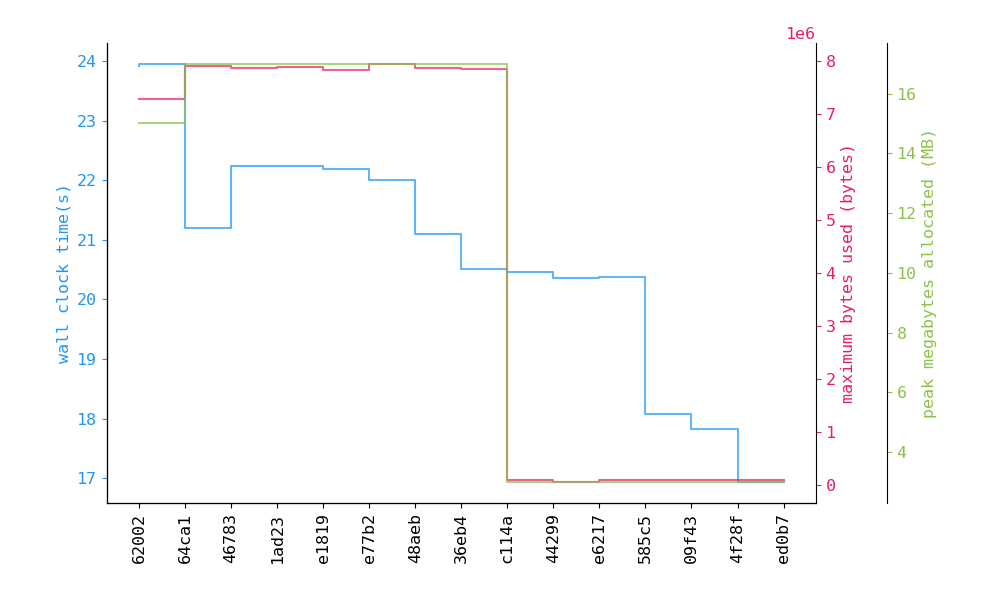
\includegraphics[height=0.6\textwidth]{./perfdata-gen.png}
\end{center}
\note[item]{\textbf{D}}
\end{frame}

\begin{frame}[fragile]{Avoid CPU ieee754 slow paths}
\begin{minted}{hs}
 intersect :: Ray -> Sphere -> Double
 intersect (Ray o d) (Sphere r p _e _c _refl) =
   if det<0
-  then 1/0.0
+  then 1e20
   else
    ...
-    in if a>eps then a else if s>eps then s else 1/0.0
+    in if a>eps then a else if s>eps then s else 1e20
 
...
 radiance :: Ray -> Int -> Erand48 Vec
 radiance ray@(Ray o d) depth = case intersects ray of
-  (T t _) | t == 1/0.0 -> return 0
+  (T 1e20 _) -> return 0
   ...
\end{minted}

\note[item]{\textbf{D}}
\note[item]{We used +Inf to match the Maybeness}
\note[item]{C++ code set 1e20 s the horizon}
\note[item]{Mechanical sympathy is important.}
\note[item]{Know how the CPU (abstractly) executes - slow path / fast path.}
\end{frame}


\begin{frame}[fragile]{Fix differences with C++ version}
\begin{minted}{diff}
-                  if depth>2
+                  if depth'>2 -- depth' = depth + 1
...
\end{minted}
\note[item]{\textbf{S}}
\note[item]{Since the sha1 of the output didn't match the C++ version we started investigating.}
\note[item]{clang++, g++ actually produce different sha1s}
\note[item]{unincremented depth was being used in one branch, causing us to do more work}
\note[item]{now confident to say we're doing the same computation as C++}
\end{frame}


\begin{frame}[fragile]{A second view from the mountaintop}
\end{frame}


\begin{frame}[fragile]{Takeaways}
\begin{itemize}
\item The unrolling in 'intersects' is ugly.
\item (We feel) the maintainability of this code hasn’t been significantly harmed.
\item We're faster than clang++ and within 6\% of g++
\item Haven't exhausted the optimization opportunities.
\item GHC could learn to do several of these optimizations for us.
\item Others are just good Haskell style. 
\item Clean Haskell is often performant Haskell.
\iten Repository stepping through each optimization is available at ...
\end{itemize}
%\item \href{https://docs.google.com/spreadsheets/d/1YhZlDRGvnCtN8UQf_0ItmgRWI9MhL21HDTlBEKqgWHc/edit#gid=0}{Raw Google Sheet of our transformations}
%\item \href{https://github.com/bollu/smallpths}{\texttt{github.com/bollu/smallpt-opt}}

\note[item]{\textbf{D}}
\end{frame}

\begin{frame}[fragile]{Raw data}
\end{frame}

\begin{frame}[fragile]{Experimental data}
\begin{itemize}
\item All test were on an otherwise idle \texttt{Equinix Metal c3.small.x86} (\texttt{Intel Xeon E-2278G} with \texttt{32GiB} RAM, Ubuntu \texttt{20.04}).
\end{itemize}
\end{frame}
\end{document}
